\chapter{Energia elettrostatica}

Analizziamo il significato dell'energia potenziale elettrostatica di un sistema di cariche. \\

Supponiamo, per semplicità, di considerare un sistema discreto di cariche. 

\begin{figure}[h]
    \centering
    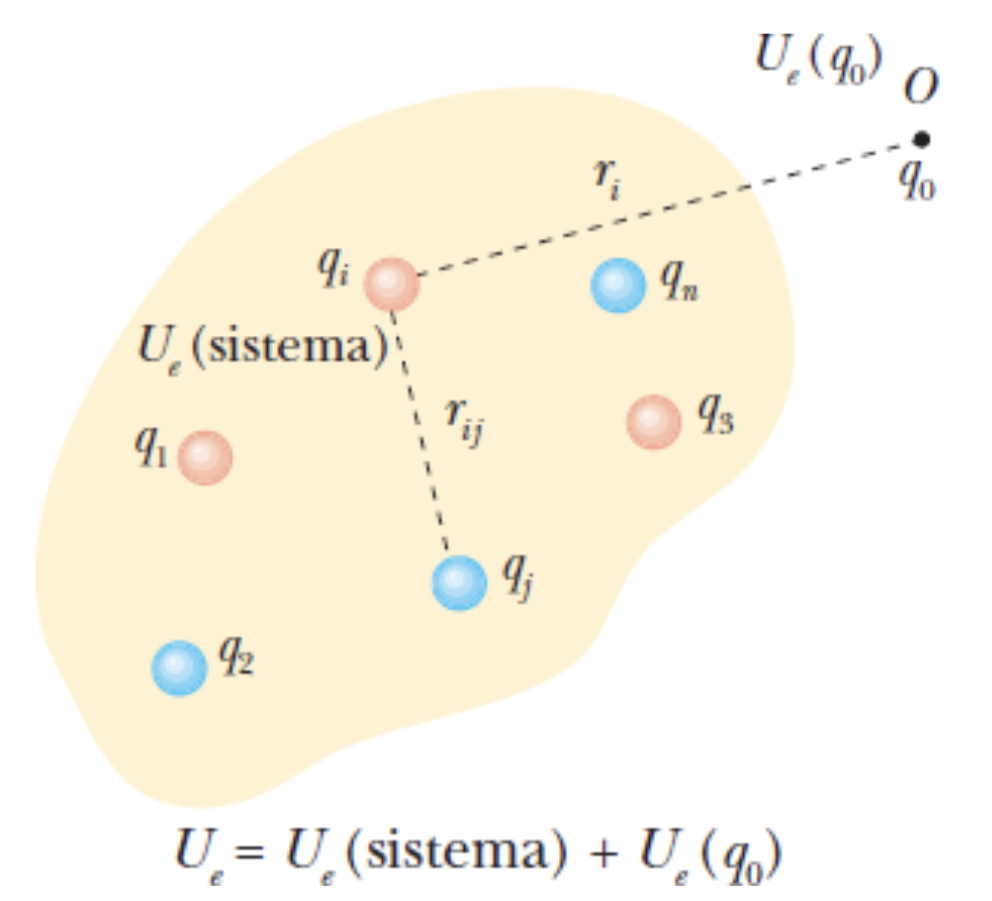
\includegraphics[width=0.47\linewidth]{figure/image5.png}
    \label{fig:chapter_5_1}
\end{figure}

Troviamo il lavoro necessario per creare questa distribuzione. Immaginiamo di portare le cariche una per una da una distanza infinita fino al suo punto nella distribuzione. Per la prima carica non ci sarà bisogno di compiere lavoro in quanto su di essa non agisce ancora nessun campo. Portando la seconda, sfruttando la \ref{eq:potenziale_per_più_cariche}, si dovrà fare un lavoro 

\begin{equation*}
    W_2 = \frac{1}{4 \pi \varepsilon_0} q_2 \left(\frac{q_1}{r_{12}}\right)
\end{equation*}

Dove $r_{12}$ è la distanza tra la prima e la seconda carica nella distribuzione. Portando la terza carica si ha 

\begin{equation*}
    W_3 = \frac{1}{4 \pi \varepsilon_0} q_3 \left( \frac{q_1}{r_{13}} + \frac{q_2}{r_{23}} \right)
\end{equation*}

In questo modo si capisce che per portare la carica j-esima si dovrà fare un lavoro 

\begin{equation}
    W_j = \frac{1}{4 \pi \varepsilon_0} q_j  \sum_{i=1} ^ {j-1}  \frac{q_i}{r_{ij}}
\end{equation}

Ma allora il lavoro totale sarà dato dalla somma di tutti questi lavori, quindi 

\begin{equation}
    W = \frac{1}{4 \pi \varepsilon_0} \sum_{i = 1} ^n \sum_{j>1}^n \frac{q_i  q_j}{r_{ij}}
\end{equation}

Dove la condizione $j>i$ è per non contare lo stesso paio di cariche due volte. Un modo migliore, allora, è quello di contare tutte le coppie di cariche due volte e poi dividere per due 

\begin{equation}
    W = \frac{1}{8 \pi \varepsilon_0} \sum_{i = 1} ^ {n} \sum_{j \neq i} ^n \frac{q_i q_j}{r_{ij}}
\end{equation}

Allora portando fuori dalla seconda sommatoria i termini che non dipendono da $j$, otteniamo 

\begin{equation}
    W = \frac{1}{2} \sum_{i = 1} ^n q_i \left( \sum_{j \neq i}^n \frac{1}{4 \pi \varepsilon_0} \frac{q_j}{r_{ij}} \right)
\end{equation}

Si nota che i termini in parentesi rappresentano il potenziale che agisce sulla carica j-esima una volta raggiunta la distribuzione, pertanto si ha che il lavoro totale necessario per ottenere la distribuzione è 

\begin{equation}
    W = \frac{1}{2} \sum_{i = 1}^n q_i V(\mathbf{r}_i)
\end{equation}

Ma questo lavoro rappresenta anche l'energia che il sistema accumula, quindi possiamo dire che l'energia elettrostatica del sistema è proprio 

\begin{tcolorbox}[colback=yellow!10!white, colframe=orange!70!black, boxrule=0.8pt]
\begin{equation}
    U_e = \frac{1}{2} \sum_{i \neq j} \frac{q_i q_j}{4 \pi \varepsilon_0 r_{ij}} = \frac{1}{2} \sum_{i = 1}^n q_i V(\mathbf{r}_i)
    \label{eq:energia_elettrostatica_discreto}
\end{equation}
\end{tcolorbox}

\section{Energia elettrostatica per una distribuzione continua}

Per una distribuzione continua di carica di densità di carica $\rho$ la \ref{eq:energia_elettrostatica_discreto} diventa

\begin{tcolorbox}[colback=yellow!10!white, colframe=orange!70!black, boxrule=0.8pt]
\begin{equation}
    U_e = \frac{1}{2} \int V dq = \frac{1}{2} \int_{\tau} \rho V \ d\tau
    \label{eq:energia_elettrostatica_continuo}
\end{equation}
\end{tcolorbox}

Tuttavia possiamo esprimere questo risultato in un'altra forma molto utile.\\
Sfruttando il teorema di Gauss in forma locale si ha 

\begin{equation*}
    \rho = \varepsilon_0 \nabla \cdot \mathbf{E} \implies U_e = \frac{\varepsilon_0}{2} \int_{\tau} (\nabla \cdot \mathbf{E}) V \ d \tau
\end{equation*}

Integrando per parti ed applicando il teorema della divergenza, otteniamo

\begin{equation}
    U_e = \frac{\varepsilon_0}{2} \left[ - \int_{\tau} \mathbf{E} \cdot (\nabla V) \ d \tau + \oint_{\Sigma} V \mathbf{E} \cdot \mathbf{u}_n \ d\Sigma \right]
\end{equation}

Tuttavia $\nabla V = - \mathbf{E}$, quindi 

\begin{equation}
    U_e = \frac{\varepsilon_0}{2} \left[  \int_{\tau} E^2 \ d \tau + \oint_{\Sigma} V \mathbf{E} \cdot \mathbf{u}_n \ d\Sigma \right]
\end{equation}

Ma su quale volume stiamo integrando adesso? Dalla \ref{eq:energia_elettrostatica_continuo} è chiaro che stiamo integrando sul volume della distribuzione, in realtà, però, andrebbe bene qualsiasi volume più grande contenente la distribuzione, in quanto tutto il volume in "eccesso" non darebbe alcun contributo all'integrale, dato che all'esterno della distribuzione $\rho = 0$. \\

Vediamo cosa succede quando andiamo a considerare volumi sempre più grandi. L'integrale contenente il termine $E^2$ può andare solo ad aumentare, questo implica che il secondo integrale deve andare a diminuire, per mantenere la quantità costante. \\

Si nota in questo modo che se andiamo a integrare in \emph{tutto lo spazio} allora si andrà ad annullare in contributo del secondo integrale e quindi avremo 

\begin{tcolorbox}[colback=yellow!10!white, colframe=orange!70!black, boxrule=0.8pt]
\begin{equation}
    U_e = \frac{\varepsilon_0}{2} \int E^2 \ d \tau
\end{equation}
\label{eq:energia_elettrostatica_campo}
\end{tcolorbox}

Dobbiamo fare sempre attenzione ad integrare su tutto lo spazio. 
